\documentclass{article} % 文書クラスの指定
\usepackage[dvipdfmx]{graphicx}	      %	図を取り込む		   (推奨)
\usepackage{enumitem}                 %	箇条書きを変更する
% \usepackage{caption}                  % caption パッケージの追加
% \captionsetup[figure]{labelsep=} % 図のキャプションの形式を "図6.1(スペース)" に設定
% \captionsetup[table]{labelsep=space}  % 表のキャプションの形式を "表6.1(スペース)" に設定
\usepackage{color}                    % いろいろな色を使えるようにする
\usepackage{url}                      % URLを使えるようにする
\usepackage[left=20mm,right=20mm]{geometry}

% \usepackage{plistings}      % listingsパッケージをpLaTeX上で用いる際の日本語対応処理を強化するためのパッケージ.(plistings.sty)を同一ディレクトリに配置.

\title{音響信号への遅延生成アプリケーション Readme} % 文書のタイトル
\author{知能信号処理研究室\\\\山下一樹} % 著者名
% 所属
\date{\today} % 日付

\begin{document} % 文書の開始
\maketitle % タイトル、著者名、日付の表示
本稿は、客観調査のためのアプリケーションを使用するための説明書である。
\section{各要素の説明} 
図\ref{fig:app_kyakkann}にアプリケーションの画面を示す。
以下に赤色の点線で囲った各要素について説明する。
\begin{figure}[tbp]
  \centering
  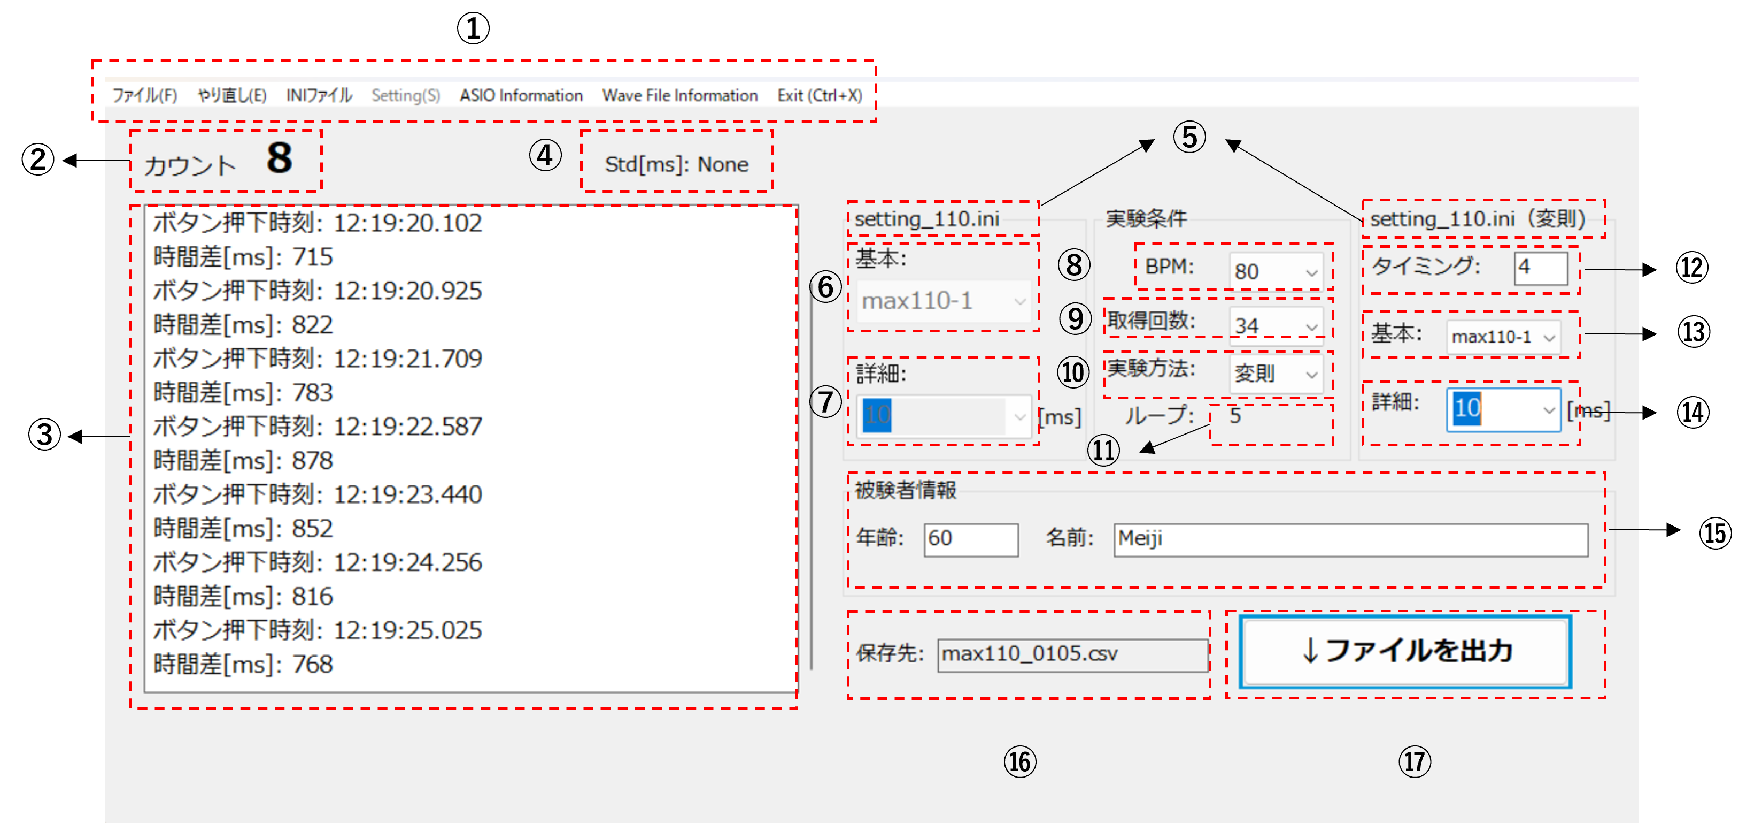
\includegraphics[scale=0.5]{figures_app_1.pdf}
  \caption{アプリケーションの画面}
  \label{fig:app_kyakkann}
\end{figure}
\begin{enumerate}
  \item メニューバー。アプリケーションの操作に関するメニューが表示される。
  「ファイル」は、結果を保存するためのCSVファイルを選択するためのメニューである。
  「やり直し」は、ボタンの押下回数をリセットするためのメニューである。
  「INIファイル」は、遅延時間が記述されているiniファイルを選択するメニューである。このiniファイルは指定されたフォルダ内に保存されていなければならない。詳細は2章を参照。
  \item ボタンの押下回数を表示する。
  \item ボタンの押下時刻と前回押した時刻のとの差[ms]を表示する。 
  \item ボタンの押下間隔[ms]のデータの標準偏差を表示する。外れ値を含むすべてのデータの標準偏差を表示する。
  分析データとしてはこの値は使用しない。
  \item 設定したiniファイル名を表示する。
  \item 指定したiniファイルに記述された遅延時間のグループ名を表示するコンボボックス。
  \item (6)で選択された遅延時間のグループ名の遅延時間[ms]を表示するコンボボックス。
  \item CSVファイルに出力するBPMの値を指定するためのコンボボックス。デフォルトは80。
  \item ボタンの押下間隔の取得回数を指定するためのコンボボックス。デフォルトは34。(2)がここで指定した回数に到達すると、
  メッセージボックスが出力され音の出力が一時的に停止する。
  \item 実験方法を指定するためのコンボボックス。デフォルトは「変則」。
  変則に設定すると、右側のコンボボックスが有効化される。通常の場合、(7)で設定した遅延時間で音が毎回出力される。
  変則の場合、(12)で指定した倍数に到達すると音声に遅延が(14)で指定した遅延時間だけ加えられる。それ以外の場合は、(7)で指定した遅延時間だけ加えられた音声が出力される。
  \item プログラム中で設定するfor分のループ回数。この値が小さい程遅延時間が小さい。アプリ開発中に使用していたため、現在は使用していない。
  \item 遅延のタイミングを指定するためのエディットボックス。デフォルトは4。ここで指定された値の倍数に(2)が到達すると音声に遅延が(14)で指定した遅延時間だけ加えられる。
  \item (1)で設定したiniファイルのグループ名を指定するためのコンボボックス。
  \item (13)で指定したグループの遅延時間[ms]を指定するためのコンボボックス。
  \item 被験者の情報を入力するためのエディットボックス。ここに書かれた情報もCSVファイルに書き込まれる。
  後続のデータ分析などに利用される。
  \item (1)で選択したCSVファイルの名前を表示する。
  \item 結果を保存するためのプッシュボタン。押下すると、(1)で指定したファイル名でCSVファイルが保存される。(10)で指定した実験方法により、書き込むデータの内容が若干異なる。
\end{enumerate}

\section{INIファイルの設定}
アプリケーションがiniファイルに記述された遅延時間を読み込むために、exeファイルと同じフォルダ内に、
「setting」という名前のフォルダを作成し、その中に遅延時間を記述したiniファイルを保存する必要があります。
setting\_110.iniファイルに遅延時間を設定して置くことができます。iniファイルはテキストエディタで編集可能です。
以下にiniファイルの例を示します。
まず、「setting」セクション内の「latedataname」キーに遅延時間のグループ名を設定します。
次に、設定した遅延時間のグループ名のセクションを作成し、「data」キーにカンマ区切りで遅延時間を設定します。
これを行うとアプリケーションで遅延時間を読み込むことができます。

\section{改善点}
\begin{enumerate}
  \item iniファイルのデフォルト名が「setting\_110.ini」になっている。そのため、決まったフォルダ内に「setting\_110.ini」が保存されていなければならない。
  \item 音声の出力先のチャンネル数を指定できるようにする。
  \item ボタンの押下回数が指定された回数に到達したときに、メッセージボックスによって強制的に音声の出力を一時的に停止する機能があるが、
  メッセージボックスを閉じた直後に音声が出力されないようにしたい。
\end{enumerate}
\end{document} % 文書の終了
